% This is "sig-alternate.tex" V2.1 April 2013
% This file should be compiled with V2.5 of "sig-alternate.cls" May 2012
%
% This example file demonstrates the use of the 'sig-alternate.cls'
% V2.5 LaTeX2e document class file. It is for those submitting
% articles to ACM Conference Proceedings WHO DO NOT WISH TO
% STRICTLY ADHERE TO THE SIGS (PUBS-BOARD-ENDORSED) STYLE.
% The 'sig-alternate.cls' file will produce a similar-looking,
% albeit, 'tighter' paper resulting in, invariably, fewer pages.
%
% ----------------------------------------------------------------------------------------------------------------
% This .tex file (and associated .cls V2.5) produces:
%       1) The Permission Statement
%       2) The Conference (location) Info information
%       3) The Copyright Line with ACM data
%       4) NO page numbers
%
% as against the acm_proc_article-sp.cls file which
% DOES NOT produce 1) thru' 3) above.
%
% Using 'sig-alternate.cls' you have control, however, from within
% the source .tex file, over both the CopyrightYear
% (defaulted to 200X) and the ACM Copyright Data
% (defaulted to X-XXXXX-XX-X/XX/XX).
% e.g.
% \CopyrightYear{2007} will cause 2007 to appear in the copyright line.
% \crdata{0-12345-67-8/90/12} will cause 0-12345-67-8/90/12 to appear in the copyright line.
%
% ---------------------------------------------------------------------------------------------------------------
% This .tex source is an example which *does* use
% the .bib file (from which the .bbl file % is produced).
% REMEMBER HOWEVER: After having produced the .bbl file,
% and prior to final submission, you *NEED* to 'insert'
% your .bbl file into your source .tex file so as to provide
% ONE 'self-contained' source file.
%
% ================= IF YOU HAVE QUESTIONS =======================
% Questions regarding the SIGS styles, SIGS policies and
% procedures, Conferences etc. should be sent to
% Adrienne Griscti (griscti@acm.org)
%
% Technical questions _only_ to
% Gerald Murray (murray@hq.acm.org)
% ===============================================================
%
% For tracking purposes - this is V2.0 - May 2012

\documentclass{sig-alternate-05-2015}

\usepackage{etoolbox}
\makeatletter
\patchcmd{\maketitle}{\@copyrightspace}{}{}{}
\makeatother

\begin{document}

% Copyright
%\setcopyright{acmcopyright}
%\setcopyright{acmlicensed}
%\setcopyright{rightsretained}
%\setcopyright{usgov}
%\setcopyright{usgovmixed}
%\setcopyright{cagov}
%\setcopyright{cagovmixed}


% DOI
\doi{10.475/123_4}

% ISBN
\isbn{123-4567-24-567/08/06}

%Conference
\conferenceinfo{PLDI '13}{June 16--19, 2013, Seattle, WA, USA}

\acmPrice{\$15.00}

%
% --- Author Metadata here ---
\conferenceinfo{WOODSTOCK}{'97 El Paso, Texas USA}
\CopyrightYear{2007} % Allows default copyright year (20XX) to be over-ridden - IF NEED BE.
\crdata{0-12345-67-8/90/01}  % Allows default copyright data (0-89791-88-6/97/05) to be over-ridden - IF NEED BE.
% --- End of Author Metadata ---

\title{Twitter Stream Mining: analysis of  basic techniques}
%\subtitle{[Extended Abstract]
%\titlenote{A full version of this paper is available as
%\textit{Author's Guide to Preparing ACM SIG Proceedings Using
%\LaTeX$2_\epsilon$\ and BibTeX} at
%\texttt{www.acm.org/eaddress.htm}}}
%
% You need the command \numberofauthors to handle the 'placement
% and alignment' of the authors beneath the title.
%
% For aesthetic reasons, we recommend 'three authors at a time'
% i.e. three 'name/affiliation blocks' be placed beneath the title.
%
% NOTE: You are NOT restricted in how many 'rows' of
% "name/affiliations" may appear. We just ask that you restrict
% the number of 'columns' to three.
%
% Because of the available 'opening page real-estate'
% we ask you to refrain from putting more than six authors
% (two rows with three columns) beneath the article title.
% More than six makes the first-page appear very cluttered indeed.
%
% Use the \alignauthor commands to handle the names
% and affiliations for an 'aesthetic maximum' of six authors.
% Add names, affiliations, addresses for
% the seventh etc. author(s) as the argument for the
% \additionalauthors command.
% These 'additional authors' will be output/set for you
% without further effort on your part as the last section in
% the body of your article BEFORE References or any Appendices.

\numberofauthors{3} %  in this sample file, there are a *total*
% of EIGHT authors. SIX appear on the 'first-page' (for formatting
% reasons) and the remaining two appear in the \additionalauthors section.
%
\author{
% You can go ahead and credit any number of authors here,
% e.g. one 'row of three' or two rows (consisting of one row of three
% and a second row of one, two or three).
%
% The command \alignauthor (no curly braces needed) should
% precede each author name, affiliation/snail-mail address and
% e-mail address. Additionally, tag each line of
% affiliation/address with \affaddr, and tag the
% e-mail address with \email.
%
% 1st. author
\alignauthor
Christina Pardalidou
     \affaddr{Department of Informatics}\\
     \affaddr{Aristotle University of Thessaloniki}\\
     \email{\{chripard@csd.auth.gr}\}
% 2nd. author
\alignauthor
Alex Tsilingiris\\
     \affaddr{Department of Informatics}\\
     \affaddr{Aristotle University of Thessaloniki}\\
     \email{\{alextsil@csd.auth.gr}\}
% 3rd. author
% 2nd. author
\alignauthor
Sotiris Karapostolakis\\
	\affaddr{Department of Informatics}\\
	\affaddr{Aristotle University of Thessaloniki}\\
	\email{\{skarapost@csd.auth.gr}\}
%\alignauthor Lars Th{\o}rv{\"a}ld\titlenote{This author is the
%one who did all the really hard work.}\\
 %    \affaddr{The Th{\o}rv{\"a}ld Group}\\
%     \affaddr{1 Th{\o}rv{\"a}ld Circle}\\
 %    \affaddr{Hekla, Iceland}\\
 %    \email{larst@affiliation.org}
}

\maketitle
\begin{abstract}
With the advancement of web technology and its growth, there is a huge volume of data present in the web for internet users and a lot of data is generated too. Internet has become a platform for online learning, exchanging ideas and sharing opinions. Social networking sites like Twitter are rapidly gaining popularity as they allow people to share and express their views about topics, have discussion with different communities, or post messages across the world. Detecting topics in Twitter streams has been gaining an increasing amount of attention. It can be of great support for communities struck by natural disasters, and could assist companies and political parties understand users' opinions and needs. Sentiment analysis of twitter data is helpful to analyze the information in the tweets where opinions are highly unstructured, heterogeneous and are either positive or negative, or neutral in some cases. Another interesting topic regarding twitter posts is the discovery of their geolocation. The limited availability of self-identified geolocation information makes it challenging to place current and trending topics on the globe. In this paper, we present various techniques concerning all of the topics mentioned above.
\end{abstract}


%
% The code below should be generated by the tool at
% http://dl.acm.org/ccs.cfm
% Please copy and paste the code instead of the example below. 
%
%\begin{}
%<ccs2012>
 %<concept>
  %<concept_id>10010520.10010553.10010562</concept_id>
  %<concept_desc>Computer systems organization~Embedded systems</concept_desc>
  %<concept_significance>500</concept_significance>
 %</concept>
 %<concept>
  %<concept_id>10010520.10010575.10010755</concept_id>
  %<concept_desc>Computer systems organization~Redundancy</concept_desc>
  %<concept_significance>300</concept_significance>
 %</concept>
 %<concept>
  %<concept_id>10010520.10010553.10010554</concept_id>
  %<concept_desc>Computer systems organization~Robotics</concept_desc>
  %<concept_significance>100</concept_significance>
 %</concept>
 %<concept>
  %<concept_id>10003033.10003083.10003095</concept_id>
  %<concept_desc>Networks~Network reliability</concept_desc>
  %<concept_significance>100</concept_significance>
 %</concept>
%</ccs2012>  
%\end{}

%\ccsdesc[500]{Computer systems organization~Embedded systems}
%\ccsdesc[300]{Computer systems organization~Redundancy}
%\ccsdesc[100]{Networks~Network reliability}


%
% End generated code
%

%
%  Use this command to print the description
%
\printccsdesc

% We no longer use \terms command
%\terms{Theory}

\keywords{Twitter, Event Detection, Sentiment Analysis, Geolocation}

\section{Introduction}
Nowadays, the World Wide Web has transformed from a large, static library that people only browse into a vast and dynamic information resource. Relying on this, social networks is a very popular and powerful tool for expressing opinions, broadcasting news, and simply communicating with friends. People using them for commenting on significant events in real time, with several hundred micro-blogs posted each second. 

The most popular micro-blogging service is Twitter. The popularity of Twitter stems from its availability on a number of different electronic devices (web and cell phones. There is a prevalence of a subculture in Twitter that encourages users to acquire a large friend pool, as well as send tweets on a wide variety of subjects, typically several times a day. 

Monitoring and analysing this rich and continuous flow of user-generated content can yield unprecedentedly valuable information, which would not have been available from traditional media outlets. Tweets can be seen as a dynamic source of information enabling individuals, corporations, and government organizations to stay informed of "what is happening now." For instance, people would be interested in getting advice, opinions, facts, or updates on news or events\cite{petrovic2010streaming}. Companies are increasingly using Twitter to advertise and recommend products, brands, and services; to build and maintain reputations; to analyse users' sentiment regarding their products (or those of their competitors); to respond to customers' complaints; and to improve decision making and business intelligence. Twitter has also emerged as a fast communication channel for gathering and spreading breaking news, for predicting election results, and for sharing political events and conversations. It has also become an important analytical tool for crime prediction and monitoring terrorist activities.

Twitter promotes an attractive style stating breaking news, as there is very little lag\cite{Sankaranarayanan2009TwitterStandNI} between the time that an event happens or is first reported in the news media and the time at which it is the subject of a posting on Twitter. Twitter can be characterized as an endless database, which collects millions of real-time short text messages every second. Tweets also have a mechanism by which the user can link to other objects on the web such as articles, images or videos which is typically used to link tweets to related material on the Internet. Thereafter, the first result is that the size of information is multiplied and the variety of references is bigger, as well. These messages are not only just data, but they can be manipulated efficiently. One well-timed subject of research is to use those messages for event detection. In other words, the tweets is a source of inventing which topics are more seasonable. Event detection has also instant impact on the world, through the quick transmission of the news and necessary briefing in some cases. 

With the passage of time and the effect of more and more users the topic acquire much popularity. Through this phenomenon we can form a general summarization of the event. This process is called event summarization. The massive crowd keeps close pace with the development of trending topics and provide the timely updated information. Twitter has shown its powerful ability in information delivery in many events, like the wildfires in San Diego and the earthquake in Japan\cite{gao2013sequential}. In response to searches for ongoing events, today's major search engines simply find tweets that match the query terms, and present the most recent ones. This approach has the advantage of leveraging existing query matching technologies, and for simple one-shot events such as earthquakes it works well. However, for events that have "structure" or are long-running, and where users are likely to want a summary of all occurrences so far, this approach is often unsatisfactory.

Event detection is a growing domain of research. Many different species of algorithms have been detected regarding this sector. A common approach are techniques that are based on text categorization. In addition, there are some methods that reclaim the display frequency of each term.

The computational treatment of sentiment has recently attracted a great deal of attention, in part because of its potential applications. One of the main reasons for sentiment analysis is the aforementioned increase of user-generated content on the Web which has resulted in a wealth of information that is potentially of vital importance to institutions and companies. Typically, document-based sentiment analysis processes operate at a particular level, i.e. at the word or sentence level, for extracting a document's sentiment. In machine learning, the most popular approach for sentiment analysis, the selection of appropriate features for representing a document is crucial. In sentiment identification at the word level different types of features have been introduced, which are either sentiment-based (e.g. words which express a specific sentiment), syntactic-based (e.g. part-of-speech and n-grams)\cite{chatzakou2015multispot}, or semantic-based (e.g. semantic word vector spaces which capture the meaning of each word).

Document-level polarity classification is not a special case of text categorization with sentiment -rather than topic- based categories. Hence, standard machine learning classification techniques, such as support vector machines (SVMs) \cite{pang2004sentimental}, can be applied to the entire documents themselves. Nevertheless, some researches presented a technique that it is easy to improve the accuracy, by integrating sentence-level subjectivity detection with document-level sentiment polarity.

As we know, in the machine learning approach, each classifier is trained using a collection of representative data. In contrast, the semantic-orientation approach does not require prior training; instead, it measures a word containing positive or negative sentiment. Each approach has its own benefits and drawbacks. For example, the machine learning approach tends to be more accurate, but the semantic-orientation approach has better generality\cite{dang2010lexicon}. Recently, a new lexicon-enhanced method was accrued to generate a set of sentiment words based on a sentiment lexicon as a new feature dimension. It combines these sentiment features with content-free and content-specific features used in the existing machine-learning approach. In the evaluation stage, they showed that adding the new set of sentiment features can increase sentiment-classification performance.

The Internet and other communication technologies play a potentially disruptive role on the constraints imposed on social networks. These technologies reduce the overhead and cost for being introduced to new people regardless of geography, and help us stay in touch with those we know. Some have even gone so far as to call this "the end of geography", where the process of relationship formation becomes disentangled from distance altogether.

However, geography still plays an important role. The reason is because of the strong relationship between event detection and geographical location each user belongs. Twitter is a social networking website, which means that users need not be viewed in isolation, but instead can be viewed as part of a large network of other users, user groups, and user cliques. Moreover, users have some meta-data information, such as description, source location, friends, which means that the social network structure in Twitter can aid in finding users that are most likely to tweet about news belonging to a particular geographic location or region.

The rise of micro-blogging services spurred various applications to mine the data coming from those services\cite{mahmud2012tweet}. Many such applications could benefit from information about the location of users, but unfortunately location information is currently very sparse. The main problem is that less than 1 per cent of tweets are geo-tagged and information available from the location field in users' profiles is unreliable at best. The benefits of mining those data promises new personalized information services, including local news summarized from tweets of nearby Twitter users, the targeting of regional advertisements, spreading business information to local customers, and novel location-based applications (e.g., Twitter-based earthquake detection, which can be faster than through traditional official channels).

There is a great number of geoinference using social networks One direction has produced approaches that claim to accurately locate the majority of posts within tens of kilometres of their true locations\cite{han2014text}. Another method predicts the location of an individual from a sparse set of located users with peformance that exceeds IP-based geolocation. On the side, there is also a technique that predicts locations of Twitter users at different granularities, such as city, state, or time zone, using the content of their tweets and their tweeting behaviour.

Getting started the first section of this survey is the presentation of some techniques that aim to event detection. The survey detects both algorithms that are based on text categorization and frequency display methods. The second chapter deals with techniques of sentiment analysis. We give more weight on techniques that use machine learning. The last chapter unfolds methods for location identification.


\section{Event Detection}
Given a series of twitter posts, the goal of event detection is to extract a particular event by analysing the text or hashtag of a tweet. The process of event detection is not a lenient task as tweets stream in huge volumes and the level of noise is kept high \cite{petrovic2010streaming}. On the other hand, the huge volume of the stream allows the use of streaming algorithms, thus making event detection an accomplishable task \cite{petrovic2010streaming}. 
\par
The conventional approach for this problem is to represent the documents as term frequency vectors \cite{petrovic2010streaming}. When a new document arrives, it is compared to all previous ones, and if its similarity to a specific document called "centroid" is below a threshold, the new document is registered as a new event \cite{petrovic2010streaming}. Unfortunately, this simple approach doesn't perform well as the dimensionality of the data expands. 
\par
Twitter's users usually tweet about their personal life, personal opinions, taste in music etc., which makes the majority of tweets unsuitable for our purpose. Although, when a noteworthy event occurs, a lot of users tweet about it. The goal of event detection is to detect these events in an automatic fashion, keeping the noise (tweets that are not events) as low as possible \cite{petrovic2010streaming}.
\subsection{Strategies for event detection}
As stated before, tweets stream in high rates and capture the pulse of the moment, therefore occupying us to process them right away \cite{Sankaranarayanan2009TwitterStandNI}. This is accomplished by using algorithms that are online in nature, meaning they can on inputs that are not known beforehand\cite{Sankaranarayanan2009TwitterStandNI}.
\par
Tweets are inherently noisy since most of them concern small user groups. In order to improve the results of event detection we first have to improve the input by extracting only useful information from noise \cite{Sankaranarayanan2009TwitterStandNI}. Even then, information that concerns us is still limited by the upper character limit set for each tweet, currently at 140 characters. Bad use of language, spelling errors and special puns also negatively affect the outcome of event detection.
\par
Twitter is an evolving platform where users come and go, and become friends and followers with each other. When designing event detection algorithms, one should keep in mind the above aspects and make the algorithms adapt well to new knowledge, otherwise watch them fail as time passes \cite{Sankaranarayanan2009TwitterStandNI}.
\par
The difference between newswire and Tweeter is that, in Tweeter, the identities of the news "reporters" in not known in advance and the news are not posted based on a schedule, but rather appear randomly among other tweets \cite{Sankaranarayanan2009TwitterStandNI}.
\subsubsection{Identifying users}
An approach to event detection is the identification of users that usually tweet about news \cite{Sankaranarayanan2009TwitterStandNI}. A technique to do this is to manually identify these users by looking for the most common set of followers among them \cite{Sankaranarayanan2009TwitterStandNI}.
Another technique to do this is to assume that a user with a high amount of followers represents an influential event source into a social community \cite{cataldi2013personalized}. As an example, we present figure \ref{fig:obama} , which features Barack Obama as the most influential node in this group \cite{cataldi2013personalized}.

\begin{figure}[h]
	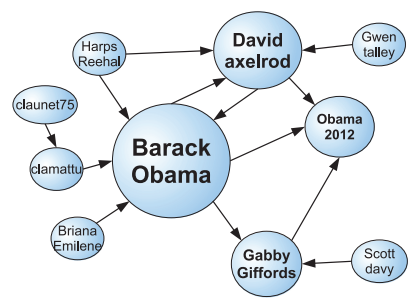
\includegraphics[scale=0.7]{obama}
	\caption{Graph showing user importance on Twitter, based on the number of their followers. \cite{cataldi2013personalized}}
	\label{fig:obama}
\end{figure}

The added benefit of this method is that, not only we identify the users of interest but, we get an evaluation of a user's influence, meaning that an influential user can affect other users' tweet streams \cite{cataldi2013personalized}. This technique cascades as the follow-like relationships spread, making it comparable to the PageRank algorithm \cite{cataldi2013personalized}.
An interesting fact to support the above claims is that studies have shown that 10\% of Twitter's users are responsible for 90\% of the tweets \cite{Sankaranarayanan2009TwitterStandNI}.

\subsection{Term and Topic Extraction}
Although manual techniques exists, we will solely focus on automatic extraction techniques as they fit best on the Twitter paradigm. Filtering could be applied on all tweets, expect those posted by influential users that usually post news, leaving us with a guaranteed source of news. The goal of the extraction is to find a way to distinguish tweets that are clearly not news, and not completely eliminate the noise, which is an enormous task to take on \cite{Sankaranarayanan2009TwitterStandNI}. For the above task, \cite{Sankaranarayanan2009TwitterStandNI} used a naive Bayes classifier that was trained using tweets that were marked as news or not news.
\subsubsection{Setting a threshold for term extraction}
An approach to selecting emerging terms relies on a user-specified threshold parameter, as described by \cite{cataldi2013personalized}. It is assumed that, given two keywords that are likely to be news, they can be considered as such based on user evaluation. A threshold value called critical drop is introduced, which allows the user to decide when a term is news or not.

\begin{figure}
	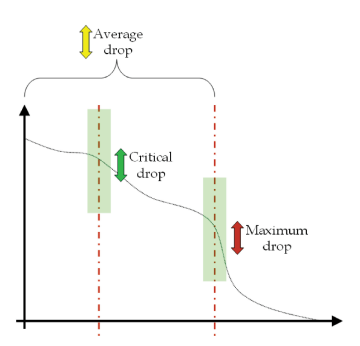
\includegraphics[scale=0.78]{criticaldrop}
	\centering
	\caption{The critical drop cut-off: the maximum drop is the highest variation in the ordered list of weights
		(red mark). The average drop (between consecutive entities) is the average difference between those items
		that are ranked before the identified maximum drop point (yellow mark). The first drop which is higher than
		the computed average drop is called the critical drop (green mark). Figure also taken from \cite{cataldi2013personalized}.}
	\label{fig:criticaldrop}
\end{figure}

In order for the above technique to work, a proper drop value has to be set. This a be a daunting task for a user or a machine. The difficulty lies in the fact that it's difficult to quantify a threshold given an abstract context that is, on top of other things, unstable. An automatic way of doing this, as described by \cite{cataldi2013personalized}, is shown below: The main idea is to preserve terms with high frequencies but only consider those whose frequency is higher than the average frequencies of most discussed terms. A model is introduced that works as follows:
\begin{itemize}
	\item Terms are ranked in descending order based on their frequencies
	\item The maximum drop value between consecutive entries is calculated and the drop point is identified.
	\item The average drop between consecutive entities for all those keywords that are ranked before the identified maximum drop point is calculated.
	\item The first drop which is higher than the computed average drop is identified as the critical drop.
\end{itemize}

At the end of this procedure, the terms ranked before the critical drop are defined as news on the specified time interval.

\subsubsection{Clustering}
The goal of clustering techniques is to group news tweets such that each group contains tweets about a specific news topic. This problem is similar to clustering documents with the main difference that the identity of news topics is not known beforehand \cite{Sankaranarayanan2009TwitterStandNI}. This problem cannot be approached by static training sets, as news evolve over time in a random fashion. A clustering approach, presented by \cite{Sankaranarayanan2009TwitterStandNI}, goes as follows: Once a tweet arrives, it is added to a news cluster and remains there forever. This techniques allows for fast processing since tweets arrive at huge rates. This makes the algorithm online. Specifically, an algorithm called leader-follower clustering has been modified and used, which allowed for clustering both in content and time. Along with the clusters, a weighted list of keywords of each tweet is kept. Time is also an important aspect in this procedure: Timestamps are kept and can render a cluster inactive if its centroid is older than a specified threshold. In this case the cluster is locked and new tweets cannot be added. 
\par
Noise can greatly affect clustering techniques. Care should be taken when creating new clusters to ensure they are of good quality. A good way to ensure high quality is to only allow the creation of clusters by influential users with many followers \cite{Sankaranarayanan2009TwitterStandNI}. All tweets from other users should be able to join a cluster but not create one. Unfortunately, this approach might prevent news registration for cases where simple users report an incident first. A way to combat this situation effectively is to allow cluster creation by users, but only activate a cluster after a certain amount of tweets has been added to it, thus making the topic news-worthy \cite{Sankaranarayanan2009TwitterStandNI}.

\subsubsection{A different approach on Clustering}
As \cite{cataldi2013personalized} states, many clustering and classification strategies cannot by applies to this task due to the fact that they tend to ignore relationships among documents(tweets) related to a news event. \cite{cataldi2013personalized} proposes a metaphor where each term is seen as a living organism: A term's vitality status increases as users use it, and slowly degrades as references drop over time. The term's vitality is weighted based on the source of the tweet. As stated before, highly influential users are more likely to post high-importance news, hence allowing us to favour terms found in their tweets.

\section{Sentiment Analysis}
Sentiment analysis (SA) can be defined as a process that automates mining of attitudes, opinions, views and emotions from text, speech, tweets and database sources through Natural Language Processing (NLP)\cite{kharde2016sentiment}. Sentiment analysis involves classifying opinions in text into categories like "positive" or "negative" or "neutral". It's also referred as subjectivity analysis, opinion mining, and appraisal extraction. Twitter Sentiment Analysis (TSA) tackles the problem of analyzing the messages posted on Twitter in terms of the sentiments they express. Twitter is a novel domain
for SA and very challenging. One of the main challenges is the length limitation, according to which tweets can be up to 140 characters. In addition, the short length and the informal type of the medium have caused the emergence of textual informalities that are extensively encountered in Twitter. Thus, methods proposed for TSA should take into account these unique characteristics. The majority of TSA methods use a method from the field of machine learning, known
as classifier. Figure 3 shows the most typical TSA process.

\begin{figure}[h]
	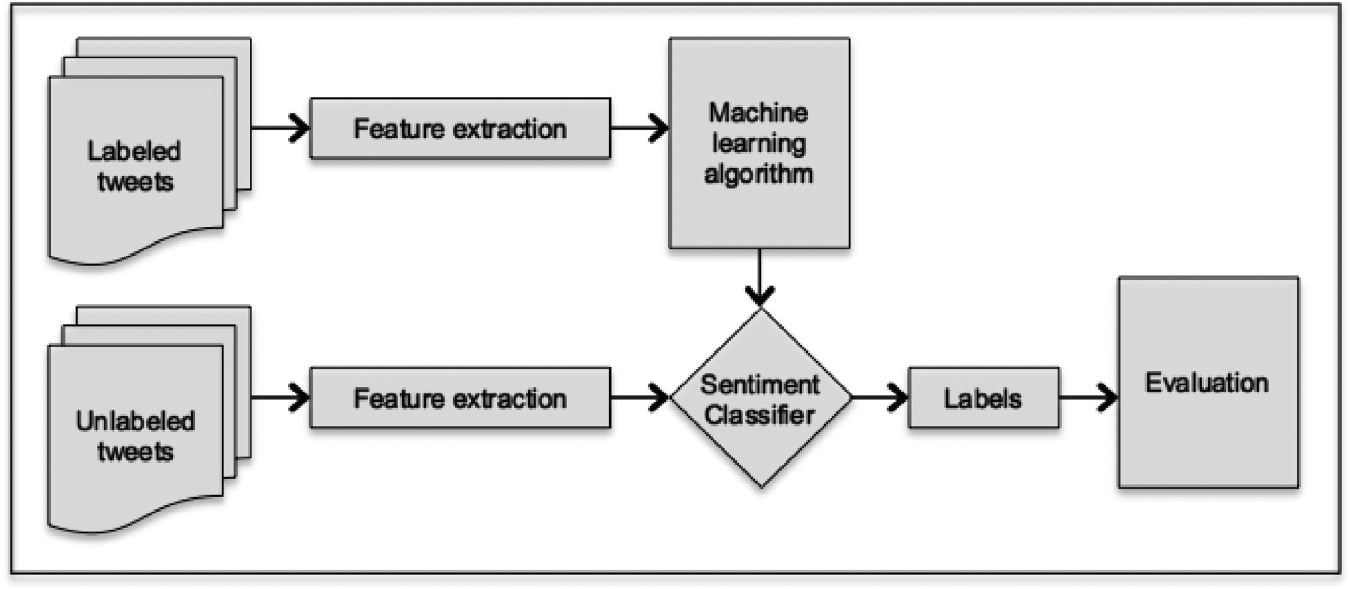
\includegraphics[scale=0.23]{sentiment-extraction}
	\centering
	\caption{Typical process for sentiment classification.  \cite{giachanou2016like}.}
	\label{fig:sentiment-extraction}
\end{figure}

\par
In the literature, SA has been applied at three different levels: \textit{document}, \textit{sentence}, and \textit{entity levels}. SA at the document level aims to identify the sentiment polarity
expressed in the whole document. The sentence level SA aims to classify each sentence as positive or negative, whereas entity-level SA detects the sentiment polarity of a
specific entity/target of a particular object.
Due to the length limitation, the majority of tweets contains a single sentence. Therefore, for the task of TSA there is no fundamental difference between document and sentence level. In case of tweets, SA can be applied on two levels: \textit{message/sentence} and \textit{entity levels}.

\begin{figure}[h]
	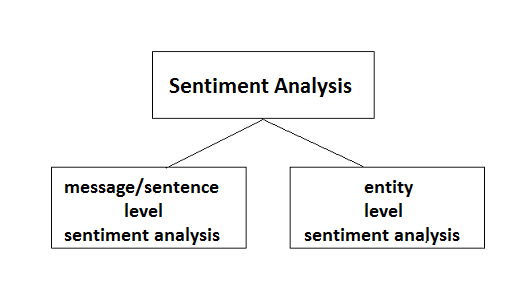
\includegraphics[scale=0.70]{schema}
	\centering
	\caption{Levels of sentiment analysis related to tweets.}
	\label{fig:schema}
\end{figure}
Four different classes can be identified in the literature of TSA:

\begin{itemize}
	\item Machine Learning
	\item Lexicon-Based
	\item Hybrid (Machine Learning and Lexicon-Based)
	\item Graph-Based
\end{itemize}

\subsection{Machine Learning}
The majority of the proposed methods that deal with TSA employs a classifier from the field of machine learning that is trained on various features of tweets. Some of the most
applied classifiers are the Naive Bayes (NB), Maximum Entropy (MaxEnt), Support Vector Machines (SVM), Multinomial Naive Bayes (MNB), Logistic Regression (LR), Random Forest (RF), and Conditional Random Field (CRF).
\par
\cite{tang2014learning} proposes learning \textit{sentiment specific word embedding} (SSWE) for sentiment analysis. It develops \textit{neural} networks and maps each \textit{ngram} to the sentiment polarity of sentence. This allows it to focus on learning the meaning of word, namely word embedding, from massive distant-supervised tweets by doing this from scratch. The effectiveness of SSWE has been implicitly evaluated by using it as features in sentiment classification on the benchmark dataset in \textit{SemEval 2013} \cite{nakov-EtAl:2013:SemEval-2013}, and explicitly verified by measuring word similarity
in the embedding space for sentiment lexicons \cite{tang2014learning}. 
\par
A deep learning approach that also uses neural networks is presented in \cite{severyn2015unitn}. This approach focuses on sentiment analysis on both message and phrase levels. The resulting model of this paper demonstrates state-of-the-art performance on both levels.
\par
One of the most used classifiers for addressing TSA is the SVM classifier. Bakliwal et al. 2012 \cite{Bakliwal:2012:MST:2392963.2392970} employed an SVM  classifier trained on 11 features to address TSA. They employed different pre-processing techniques one by one in order to measure their effectiveness. \textit{Spelling correction}, \textit{stemming}, and \textit{stop-words removal} managed to increase the accuracy of the classifier. Two different datasets were used to evaluate their approach, the Stanford dataset \cite{go2009twitter} and the Mejaj \cite{bora2012summarizing}. The best results were achieved by the combination of NLP- and Twitter-specific features.

\begin{figure}[h]
	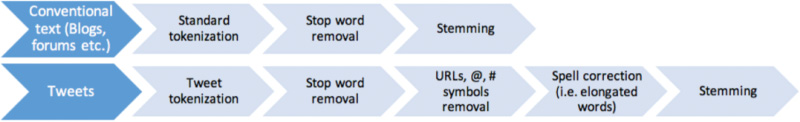
\includegraphics[scale=0.40]{tokenization}
	\centering
	\caption{Typical scenarios of preprocessing on standard text and tweets \cite{giachanou2016like}.}
	\label{fig:tokenization}
\end{figure}

\subsection{Lexicon-Based}
Lexicon-based methods leverage lists of words annotated by polarity or polarity score to determine the overall opinion score of a given text. The main advantage of these methods is that they do not require training data. Lexicon-based approaches have been extensively applied on conventional text such as blogs, forums, and product reviews. However, they are less explored in TSA compared to machine-learning methods. The main reason is the uniqueness of the text on Twitter that not only contains a large number of textual peculiarities and
colloquial expressions such as \textit{yolo} and \textit{gr8} but also has a dynamic nature with new expressions and hashtags emerging from time to time. 
\par
Ortega et al. 2013 \cite{Bueno2013SSAUOUS} proposed a three-step technique for TSA. Pre-processing was performed in the first step and polarity detection in the second step. In the last step, they performed rule-based classification. Polarity detection and rule-based classification were based on WordNet and SentiWordNet. Their approach managed to achieve good results when evaluated on the SemEval-2013 dataset \cite{nakov-EtAl:2013:SemEval-2013}. However,the authors did not compare their method with existing techniques to prove its effectiveness. \cite{dang2010lexicon} introduced some new sentiment features. The results showed that adding these newly created features, which are often used in the existing semantic-orientation approach, and the content-free and content-specific features that come from the existing machine-learning approach can improve sentiment - classification performance significantly.

\begin{figure}[h]
	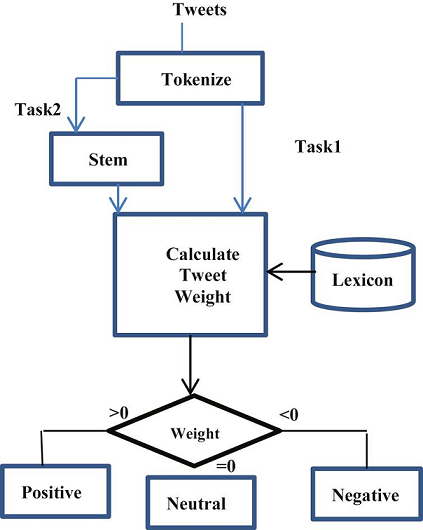
\includegraphics[scale=0.60]{lexicon-token}
	\centering
	\caption{An example of the architecture of a framework of lexicon-based sentiment analysis.}
	\label{fig:lexicon-token}
\end{figure}

\par
Another approach using a newly proposed methodology, that is lexicon-based, for capturing people's emotions in real time is presented in \cite{chatzakou2013micro}. This automated technique provides the means for an automated real-time analysis. The evaluation of the experimental results proved that the proposed method managed to capture efficiently
the emotions expressed in tweets as well as their intensity.

\subsection{Hybrid}
A number of researchers combined machine-learning and lexicon-based approaches. 
\par
An interesting hybrid method was presented by Ghiassi et al. 2013 \cite{Ghiassi:2013:TBS:2506578.2506879}, who combined dynamic artificial neural network with n-gram. Emoticons and tweets that contained the word love or hate or their synonyms were used as features to build the two classifiers: SVM and a Dynamic Architecture for Artificial Neural Networks (DAN2). The proposed approach was tested on a collection of tweets crawled using the subject \textit{Justin Bieber}. The results showed that DAN2 managed to outperform SVM.
\par
Khuc et al. 2012 \cite{Khuc:2012:TBL:2245276.2245364} also combined a lexicon-based approach with a classifier to improve TSA accuracy. They considered the MapReduce framework to create a co-occurrence
matrix based on bigram phrases. The cosine similarity between words is then computed and the edges with low cosine score are removed. Then, they combined the score generated using a simple lexicon-based approach with a classifier. For the machine learning algorithm, they used the Online LR approach. Their experiments showed that the hybrid approach outperformed the simple lexicon-based classifier that was only
based on words/phrases that indicated sentiment.
\par
Another older interesting study was presented by Zhang et al. 2011 \cite{Zhang2011CombiningLA}, who proposed a hybrid method to address entity-based TSA. For each of the entities Obama, Harry Potter, Tangled, iPad, and Packers they computed a sentiment score based on their proximity to words from a sentiment lexicon. They proposed a rule-based algorithm that also considered
\textit{comparative judgments}, \textit{negation}, and \textit{expressions} that were likely to change the orientation of a phrase. To collect more annotated data and enhance the recall of the proposed method, they identified additional subjective terms using \textit{Chi-square}. The SVM classifier was then applied for sentiment polarity detection.

\subsection{Graph-Based}
Although machine-learning methods achieve a great performance on TSA, they require a large number of annotated data. Label propagation is a method that can reduce the demand of the annotated data. For this reason, a number of researchers utilized the Twitter social graph under the assumption that people influence one another. Label propagation is a \textit{semi-supervised} method in which labels are distributed to nodes using the connection graphs.
\par
Some of the first to apply a label propagation method for TSA were Speriosu et al. 2011 \cite{Speriosu:2011:TPC:2140458.2140465}. Their proposed method leveraged the Twitter follower graph under the assumption that people influence one another. Users, tweets, unigrams, bigrams, hashtags, and emoticons were used as nodes for the construction of the graph. The proposed label propagation method outperformed a lexicon-based approach and a MaxEnt classifier.
\par
Cui et al. 2011 \cite{Cui:2011:ETB:2189339.2189365} tackled TSA with a label propagation method based on analysis of emotion tokens. At first, the emotion tokens from tweets were extracted. A graph propagation method was then used to assign polarities to the tokens. In the final
step, they analyzed and classified the emotion tokens. The emotion tokens included \textit{emoticons}, \textit{repeating punctuations}, and \textit{repeating letters}. Their approach managed to perform well in analyzing sentiment of messages written in any natural language.
\par
Instead of using emotion tokens, Wang et al. 2011 \cite{Wang:2011:TSA:2063576.2063726} proposed a graph-based model that leveraged co-occurrence of hashtags to classify the sentiment of certain hashtags. They proposed different algorithms that were compared to an SVM voting. The SVM was trained with several features, including unigrams, punctuation, and emoticons.
The Loopy Belief Propagation algorithm managed to achieve the best performance in terms of accuracy compared to the other tested methods.

\begin{figure}[h]
	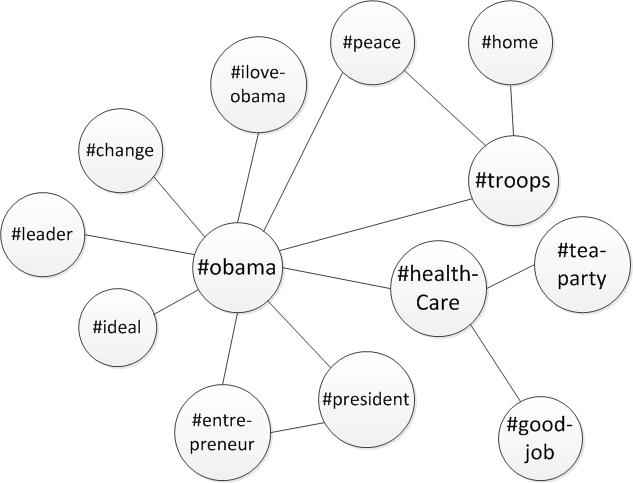
\includegraphics[scale=0.50]{hashtag}
	\centering
	\caption{An example of a Hashtag Graph Model \cite{Wang:2011:TSA:2063576.2063726} . }
	\label{fig:hashtag}
\end{figure}

\section{Geolocation Prediction}
Social media produces a continuously-updated stream of data which has proven useful for predicting group behaviors and modeling populations. Associating data with the particular geolocation from which it originated creates a powerful tool. Geo-tagged tweets would be a significant reinforcement to a variety of applications. Therefore\cite{han2014text}, recent work has focused on geoinference for predicting the locations of posts. In this section, we are going to epitomize some of the most basic techniques for Geolocation prediction.

\subsection{Prediction at Different Granularities}

A number of different kind of techniques have been recently proposed. \cite{mahmud2012tweet} propose a model whom objective is the prediction of users' location at different granularities. More specifically at city-level. The dataset for this model is consisted of 1,524,522 tweets from 9551 users. The tools for collecting the data are the Google's geocoding API, Twitter's rest API and Twitter's streaming API. Below follows the severance of the techniques to some basic categories.

\subsubsection{Content-based Statistical Classifiers}

In this part, three different models are trained. We denote as S, the set of all users' tweets. The first one uses all the words contained in S. The second one uses all hashtags that are included in S. The last one, uses all the place names that S contains. The first step is the feature selection. This process is different at each case. For the words the algorithm keeps only the nouns. For the hashtags, the algorithm keeps only the words that start with \#. The place names approach keeps only the terms that appear in the tweets and match names of US cities and states from the USGS gazetteer. Next step is the identification of terms that are particularly representative for a location. The last step is the training and classification phase. The learning algorithm that is selected is Naive Bayes Multimonial from Weka.

\subsubsection{Content-based Heuristics Classifiers}

\begin{itemize}
	\item{Local Place Heuristic Classifier:}
	The heuristic is that a user would report his or her home city or state in tweets more often than any other cities or states.
	\item{Visit Place Heuristic Classifier:}
	The heuristic is that a user would visit places in his home location more often than places in other locations.
\end{itemize}

\subsubsection{Ensemble of Location Classifiers}

The main idea in this part is a dynamically weighted ensemble of statistical and heuristic classifiers. Here we have the introduction of the Classification Strength metric. According to this, let T indicate the set of terms from user's tweets that would be considered for classification using a specific classifier. For statistical classifiers, the matching location distribution is the set of locations in our trained model containing terms from T. For the local-place classifier, this distribution contains locations from our dataset that match content in the user's tweets. For the visit-history classifier, this distribution includes locations from the user's visit history that show up in our dataset. The Classification Strength for a user is the inverse of the number of matching locations in the matching location distribution. In this approach, the Classification Strength of a classifier for a particular instance is used as the weight of that classifier in the ensemble (for classifying that instance) and the location with the highest rank by weighted linear combination is returned as the result.

For the evaluation of the classifiers, the evaluating technique is the Recall(R). The best algorithm was the Place Name Statistical Classifier. The high recall of the place name-based classifier may be explained by the fact that many users send tweets containing names of places (cities and states in our system), and those place names tend to have bias towards users' home cities.

\subsection{Network-based Geoinference}

The interest in creating new algorithms for geoinference prediction has shown a great increase. A lot of new algorithms that promise great results have been detected\cite{jurgens2015geolocation}. However, the conditions under the conclusions that was assembled are controversial. The objective of this subsection is the assessment of the state-of-the-art techniques. The three evaluating criteria are the accuracy of each algorithm in real-world conditions, (2) the impact of how ground truth is determined for training, and (3) the relationship between performance and time as models infer the locations of posts created after the model was trained. Below is the description of the 9 methods: 

\subsubsection{Techniques}

\cite{backstrom2010find} presented a model using Facebook. In this model this algorithm demands from the users to dispose highly-precised locations. The main idea of this method is the building of a probabilistic model representing the likelihood of observing a relationship between two users given the geographic distance between them. They achieved a complexity of O(|V|$k^2$ ) where V is the number of vertices in the graph and k is the average number of vertex neighbors with known locations.

\cite{mcgee2013location} proposed a method citing the difficulties adapting from Facebook to Twitter. The technique is a tree regression model that predicts the actual distance between the users. However, as the size of the network grows, computing the regression model on all pairs of located user dominates the run-time, making the algorithm unpractipable in real-world applications.

\cite{kong2014spot} proposes several extensions to the \cite{backstrom2010find} model based on strategies for weighting which of a user's friends are likely to be most predictive of their location. This method uses the friendship definition of \cite{huberman2008social} which is that a user a is friend with b if a has mentioned b in at least two posts. Given a user, their friends are weighted according to a social tightness coefficient, which is computed as the cosine similarity of the two user's friends.

\cite{li2012towards} proposes to infer geolocation by taking into account the influence of both users and of locations, capturing the intuition that some users are more informative for predicting the locations of the neighbors. The best-performing of their approaches first assigns users to random locations and then iteratively updates the locations of users from their neighbors and mentioned location names, refining the parameters in the update by measuring the prediction error of users with already-known locations.

\cite{li2012multiple} recognize that a user may relocate over the course of their social media history and therefore may have more than one home location from which they posts. To uncover all of a user's home locations, relationships between users and locations are modeled with a supervised extension to Latent Dirichlet Allocation\cite{blei2003latent}.

\cite{rout2013s} approach geolocation inference as a classification task. a SVM classifier was trained with three core features: (1) the cities of a user's friends, relative to the city's respective number of Twitter users, (2) the number of closed triads in a user's social network residing in the same city, and (3) the number of reciprocal following relationships a user has per city.

\cite{davis2011inferring} propose one of the simplest approaches where given a user, their location is inferred by
taking the most-frequently seen location among their social network.

\cite{jurgens2013s} extends the idea of location inference as label propagation by interpreting location labels spatially. Locations are inferred using an iterative, multi-pass procedure. Like \cite{kong2014spot}, during one pass, the location of each user is assigned as the geometeric median of the locations of all the user's neighbors, with groundtruth data providing the locations for the first pass.

\cite{compton2014geotagging} extend the method of \cite{jurgens2013s} to take into account edge weights in the social network and to limit the propagation of noisy locations.

\subsubsection{Evaluation Phase}

The evaluation criteria by which methods should be measured are three: (1) accurate inference of a post's location, (2) accurate inference of all the posts generated by a user, and (3) maximizing the number of posts whose location is able to be inferred. The metrics that are used for the evaluation of the techniques are three, too. Specifically, AUC, Post Coverage and Median-Max.

\begin{figure*}[h!]
	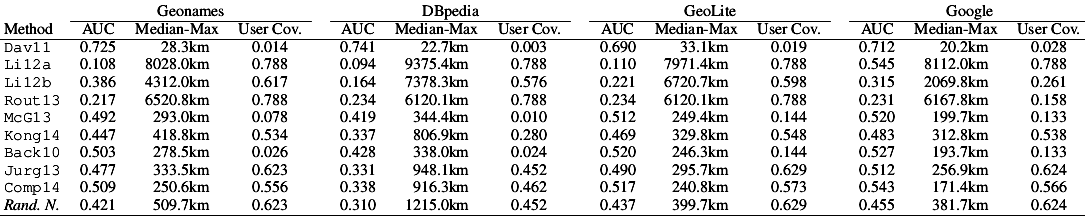
\includegraphics[width=\textwidth]{self-reported}
	\centering
	\caption{Self-reported locations identification when varying the gazetteer\cite{jurgens2015geolocation}.}
	\label{fig:reported}
\end{figure*}
\par 
The first (cross-validation) experiment is an evaluation of all nine methods and the baseline in a common setting, on identical data, using consistent sources of ground truth, and measuring performance with the proposed evaluation metrics. 

\begin{figure}[h!]
	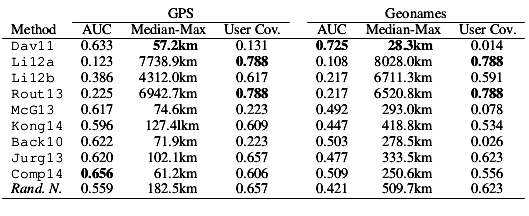
\includegraphics[scale=0.43]{cross-validation}
	\centering
	\caption{Cross-validation results of the training
		data, using different sources of ground truth\cite{jurgens2015geolocation}.}
	\label{fig:cross}
\end{figure}

\begin{figure}[h]
	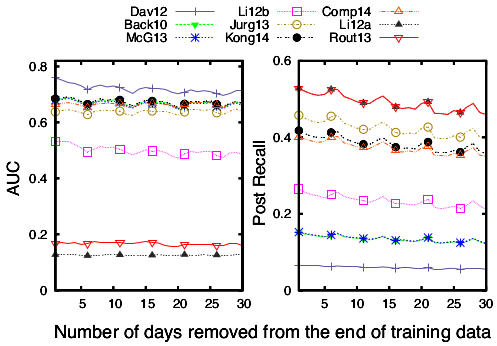
\includegraphics[scale=0.45]{temporaldecay}
	\centering
	\caption{Performance on each day of the test data\cite{jurgens2015geolocation}.}
	\label{fig:temporal}
\end{figure}


\par
The second (Self-reported Locations) experiment tests the performance impact of gazetteer choice using four, and, large gazetteers: Geonames, GeoLite, DBpedia and Google.
\par 
The last (Temporal Decay) experiment evaluates how each geoinference method changes in accuracy and coverage when predicting locations for novel Twitter data created at increasingly - distant points in time after the last date seen in the training data. Further, this experiment examines the degree to which cross-validation performance is predictive of future performance by the models.

\subsection{Prediction with Social and Spatial Proximity}

The objective of this subsection is the introduction of an algorithm that predicts the location of an individual from a sparse set of located users with peformance that exceeds IP-based geolocation\cite{backstrom2010find}.
\par 
It is observed that the likelihood of friendship with a person is decreasing with distance. This should not be surprising given that we are less likely to meet people who live further away. A less obvious relationship is that the total number of friends also tends to decrease as distance increases. This means that the probability of knowing someone d miles away is decreasing faster than the total number of people d miles away is increasing.
\par 
The model that is proposed finds that using a maximum likelihood approach with the simplifying assumption that the user will be either colocated or in close proximity to one of her friends, it is able to predict the physical location of 69.1 of the users with 16 or more located friends to within 25 miles, compared to only 57.2 using IP-based methods. The next step is to try with even more social data. The content of this data is how often users interact with each other and see each other's content. Using this data generates slight improvement in geolocation, which implies that users who are physically close to each other may tend to interact more often on Facebook. The last step is to iterate the maximum-likelihood algorithm. The reason is to increase the accuracy of prediction of many individuals at once. This showed significant improvement in the accuracy.

%ACKNOWLEDGMENTS are optional
\section{Conclusion}
Recent years have witnessed an increasing research interest in analyzing tweets. This interest is a result of the large amount of messages that are posted everyday in Twitter and that contain valuable information for a number of different topics. Event detection aims at finding real-world occurrences that unfold over space and time. As a fast-growing microblogging and online social networking service, Twitter provides
unprecedentedly valuable user-generated content that can be transformed into actionable and situational knowledge. A considerable effort is still required to achieve efficient and reliable event detection systems. Some of them are the designing of better feature extraction and query generation techniques, more accurate filtering and detection algorithms, improved techniques to combine and analyze information from multiple sources (social and traditional media) and multiple languages, and enhanced summarization and visualization approaches. As for sentiment extraction, methods from the machine-learning field are applied for TSA on a more frequent rate compared to the rest of the approaches, with the SVM and NB classifiers being the most prevalent. Unigram-based SVM is usually considered as a baseline to which the proposed methods are compared. Moreover, lexicons are utilized in a large set of proposed methods to support detecting words that indicate sentiment. SentiWordNet and MPQA are the most used lexicons that are usually extended with words that are used in Twitter. Continuing, location information on Twitter is available through geotagged tweets indicating the current location of the user at the time of tweeting. However, geotagging is not a default setting and thus rarely used. Accurate user geolocation is a key driver for location-specific services such as localised search, and has been
the target of research across different disciplines. One of the most reliable and straightforward approaches to geolocation prediction is IP-based methods, but in many contexts, it is not possible to access the IP of the device used to post content, or the IP is relatively uninformative (as is the case with, e.g. mobile devices). A new-entry algorithm finds the location of a user at different granularities. Many models were trained on this approach. The best model predicts a user's location, using as a training set only the places of a users' tweets. The location of a person can also be predicted using the activity of their friends' network. This method first analyzes friendship as a function of distance and rank and generates several observations regarding the interplay of geography and friendship. They find that at medium to long-range distances, the probability of friendship is roughly proportional to the inverse of distance. Then they present an algorithm to predict the physical location of a user, given the known location of his friends. The most interesting part is the comparison of the state-of-the-art techniques in the geolocation prediction. The authors consider that the results are under controversial conditions and in order to make right conclusions they tried a comparison among them. To conclude, since the data mining regarding the social media is at a primary stage, further work must be done in order to provide more accurate methods and techniques in the future.


\bibliographystyle{abbrv}
\bibliography{sigproc}  % sigproc.bib is the name of the Bibliography in this case
%\nocite{*} %auto einai gia na bgazei to reference xwris na xreiazetai na to kanoume cite kapou.

\end{document}
